\section{Results}\label{sec:results}

\subsection{RQ1: When do projects migrate?}\label{sec:rq1}

Table~\ref{tab:phases} places every exposed repository on the timeline of its deprecation.
For the artifact actions, only 30 of 90 repositories (33\%) migrated while nothing had broken yet, although the warning period lasted more than nine months for v3.
Four more migrated during the brownouts in January~2025, and 51 (57\%) migrated only after their workflows had started to fail.
Five never migrated.
For \so{}, 25 of 57 repositories (44\%) migrated before the announced cutoff, one in the eight weeks between the announced date and its postponement, 22 (39\%) after the postponement, and nine never did.

\begin{table}[t]
\caption{RQ1: Phase of the migration on the timeline of each deprecation}\label{tab:phases}
\centering\footnotesize
\begin{tabular}{@{}L{0.42\columnwidth}rr@{\hspace{10pt}}L{0.24\columnwidth}@{}}
\toprule
\textbf{Phase} & \textbf{Repos} & \textbf{\%} & \\
\midrule
\multicolumn{4}{@{}l}{\textit{Artifact actions v1--v3 (n = 90), enforced cutoff}} \\
Before any breakage & 30 & 33.3 & \\
During the v3 brownouts & 4 & 4.4 & \\
After the cutoff (CI broken) & 51 & 56.7 & \\
Not migrated & 5 & 5.6 & \\
\midrule
\multicolumn{4}{@{}l}{\textit{\so{} (n = 57), withdrawn cutoff}} \\
Before the announced cutoff & 25 & 43.9 & \\
Between cutoff date and postponement & 1 & 1.8 & \\
After the postponement & 22 & 38.6 & \\
Not migrated & 9 & 15.8 & \\
\bottomrule
\end{tabular}
\end{table}

Fig.~\ref{fig:weekly} shows when the migrations happened.
Artifact migrations trickle in after the notice and then pile up twice: in September~2024, when v1/v2 workflows started to fail, and around the v3 brownouts and cutoff, each time followed by a tail of repositories that repaired their CI weeks or months later.
Neither announced date left a mark.
Of the 35 repositories that used v1 or v2 at the notice and later dropped them, three did so before the announced cutoff of 30~June~2024 and four in the ten weeks during which the old versions still worked after it; eleven followed within two weeks of the first failure reports, and the remaining 17 later.
Around the first announced v3 date, 30~November~2024, the v3 migrations show no increase either.
The \so{} migrations follow the opposite shape: a burst in the first weeks after the notice, steady migration until the announced cutoff, and only a thin tail after GitHub postponed it.

\begin{figure*}[t]
\centering
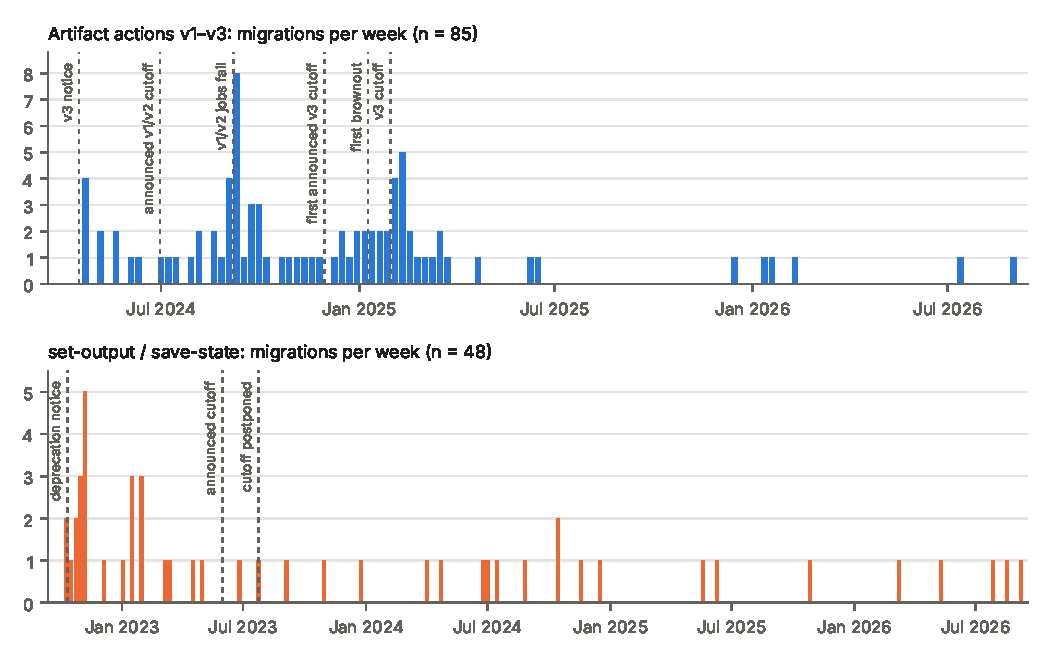
\includegraphics[width=0.9\textwidth]{figures/sample_weekly.pdf}
\caption{Migrations per calendar week. Dashed lines mark the key dates of each deprecation.}\label{fig:weekly}
\end{figure*}

\finding{1}{Warnings alone moved a minority of projects. For the enforced deprecation, 57\% of the exposed projects migrated only after their CI had broken, and migrations followed the days on which workflows actually failed, not the announced dates. For the withdrawn deprecation, migration happened mostly before the announced cutoff and nearly stopped after it was postponed.}

\subsection{RQ2: Does the way a deprecation ends matter?}\label{sec:rq2}

Fig.~\ref{fig:km} and Table~\ref{tab:survival} compare how long repositories kept using the deprecated component.
The \so{} curve falls faster at first: 19\% of the exposed repositories had migrated after 30~days, against 7\% for the artifact actions.
The picture reverses once the first artifact workflows fail: the artifact curve drops steeply in September~2024 and again around the v3 brownouts and cutoff, while the \so{} curve flattens after the postponement.
One year after the notice, 85\% of the artifact-exposed repositories had migrated, but only 49\% of the \so{}-exposed ones; the median time to migration was 224 and 384 days.
The difference is significant (log-rank $\chi^2 = 12.8$, $p < 0.001$) and remains so when non-migrants are censored at the collection date instead of their last commit ($\chi^2 = 11.3$, $p < 0.001$).

\begin{figure*}[t]
\centering
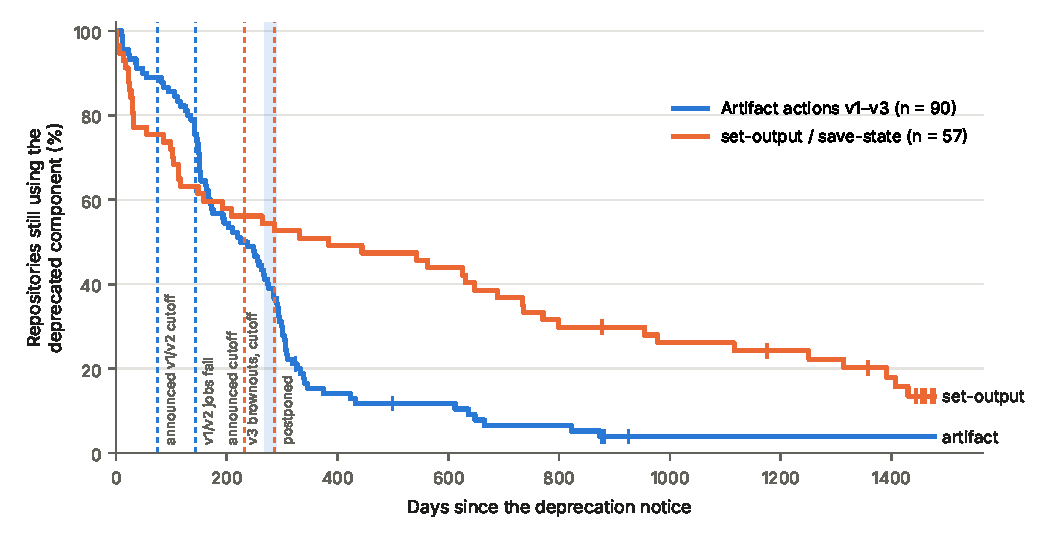
\includegraphics[width=0.9\textwidth]{figures/sample_km.pdf}
\caption{Share of exposed repositories still using the deprecated component, by days since the deprecation notice (Kaplan--Meier estimate; ticks mark censored repositories).}\label{fig:km}
\end{figure*}

\begin{table}[t]
\caption{RQ2: Time to migration (Kaplan--Meier)}\label{tab:survival}
\centering\footnotesize
\begin{tabular}{@{}lrrrrrr@{}}
\toprule
 & & \multicolumn{5}{c}{\textbf{Migrated after (\%)}} \\
\cmidrule(l){3-7}
\textbf{Event} & \textbf{Median} & \textbf{30\,d} & \textbf{90\,d} & \textbf{180\,d} & \textbf{1\,y} & \textbf{2\,y} \\
\midrule
Artifact actions & 224\,d & 6.7 & 13.3 & 43.3 & 84.8 & 93.5 \\
\so{} & 384\,d & 19.3 & 26.3 & 40.4 & 49.1 & 63.2 \\
\bottomrule
\end{tabular}
\end{table}

The two events differ in more than their ending, so we also compare the 18 repositories that migrated away from both.
Twelve of them took less time for the artifact actions than for \so{}, with a median difference of 296~days (Wilcoxon signed-rank, $p = 0.021$).
The same projects, then, reacted faster to the deprecation that was enforced.

\finding{2}{An enforced cutoff led to faster and more complete migration than a cutoff that was announced and then withdrawn (85\% vs.\ 49\% migrated within a year), also within the same projects. The withdrawn cutoff started faster but stalled once the threat disappeared.}

\subsection{RQ3: Which projects migrate in time?}\label{sec:rq3}

Projects that migrated before anything broke looked much like the others.
None of the nine characteristics we compared differed significantly after Holm's correction (Table~\ref{tab:cox}).
Two associations are suggestive.
For the artifact actions, projects that migrated in time more often had Dependabot or Renovate configured (17\% vs.\ 3\%, $p = 0.039$ uncorrected) and had been somewhat more active in the six months before the notice (median 96 vs.\ 62 commits, $p = 0.060$); in the Cox model more prior activity went with faster migration (HR 1.14 per e-fold increase).
For \so{}, projects with Dependabot or Renovate configured migrated faster (HR 2.39), although not a single \so{} migration was made by a bot (RQ4): the tools seem to mark projects that look after their CI rather than doing the work.
For both events the effect of these tools also changes over time (Schoenfeld residuals correlate with time, $\rho \approx 0.5$), so the hazard ratio is only an average.
Stars, contributors, age, the number of workflow files and the number of deprecated uses showed no association.

\begin{table}[t]
\caption{RQ3: Cox models of the time to migration}\label{tab:cox}
\centering\footnotesize
\begin{tabular}{@{}lrlrr@{}}
\toprule
\textbf{Covariate} & \textbf{HR} & \textbf{95\% CI} & \textbf{p} & \textbf{p (Holm)} \\
\midrule
\multicolumn{5}{@{}l}{\textit{Artifact actions (n = 90, 85 migrations)}} \\
Stars ($\log_{10}$) & 0.68 & 0.44--1.05 & 0.082 & 0.49 \\
Commits, 6 months before ($\log$) & 1.14 & 1.02--1.28 & 0.026 & 0.18 \\
Deprecated uses ($\log$) & 0.91 & 0.64--1.29 & 0.603 & 1.00 \\
Dependabot or Renovate & 1.87 & 0.83--4.20 & 0.130 & 0.65 \\
\midrule
\multicolumn{5}{@{}l}{\textit{\so{} (n = 57, 48 migrations)}} \\
Stars ($\log_{10}$) & 1.58 & 0.84--2.98 & 0.155 & 0.65 \\
Commits, 6 months before ($\log$) & 1.04 & 0.84--1.29 & 0.716 & 1.00 \\
Deprecated uses ($\log$) & 1.28 & 0.78--2.09 & 0.330 & 0.99 \\
Dependabot or Renovate & 2.39 & 1.21--4.72 & 0.012 & 0.10 \\
\bottomrule
\end{tabular}
\end{table}

One observation qualifies these results.
Only 5 of the 90 artifact-exposed repositories had Dependabot configured for GitHub Actions on the day of the notice.
Version~4 had been available for four months by then, so most projects with Dependabot had already been moved to it automatically and were never exposed.
Dependency bots thus act \emph{before} a deprecation, by keeping projects off outdated versions, which our design, conditioned on exposure, cannot capture.

\finding{3}{No project characteristic reliably predicts timely migration. Prior activity and the use of dependency bots point in the expected direction but do not survive correction for multiple testing. Bots mainly keep projects from being exposed in the first place.}

\subsection{RQ4: Who migrates?}\label{sec:rq4}

Table~\ref{tab:authors} shows who authored the change that removed the last deprecated use.
Core maintainers did most of the work: 74\% of the artifact migrations and 94\% of the \so{} migrations.
Bots authored only 4 artifact migrations, all of them version bumps made before anything broke, and no \so{} migration, which a version bump cannot fix.
External contributors authored 21\% of the artifact migrations.
Their share was higher before anything broke (30\%) than after the cutoff (16\%): when CI failed, maintainers fixed it themselves.

\begin{table}[t]
\caption{RQ4: Author of the migration}\label{tab:authors}
\centering\footnotesize
\begin{tabular}{@{}lrrrr@{}}
\toprule
\textbf{Event / phase} & \textbf{n} & \textbf{Bot} & \textbf{Core} & \textbf{External} \\
\midrule
\textit{Artifact actions} & 85 & 4 (5\%) & 63 (74\%) & 18 (21\%) \\
\quad before any breakage & 30 & 4 & 17 & 9 \\
\quad during the brownouts & 4 & 0 & 3 & 1 \\
\quad after the cutoff & 51 & 0 & 43 & 8 \\
\midrule
\textit{\so{}} & 48 & 0 (0\%) & 45 (94\%) & 3 (6\%) \\
\quad before the announced cutoff & 25 & 0 & 25 & 0 \\
\quad after the cutoff date & 23 & 0 & 20 & 3 \\
\bottomrule
\end{tabular}
\end{table}

\finding{4}{Migrations are maintenance work done by core maintainers. Bots contributed almost nothing once a project was exposed, and external contributors helped mostly before anything broke.}

\subsection{RQ5: How do projects migrate, and what goes wrong?}\label{sec:rq5}

Table~\ref{tab:rq5} summarizes the coding.
Most migrations were one-to-one replacements: 73\% of the artifact pairs and 60\% of the \so{} pairs.
For the artifact actions, 13\% needed further changes that v4 forced, and \so{} was more often removed or replaced by another mechanism (25\%), typically when a workflow was rewritten.

\begin{table}[t]
\caption{RQ5: Change type, trigger and problems}\label{tab:rq5}
\centering\footnotesize
\begin{tabular}{@{}lrr@{}}
\toprule
 & \textbf{Artifact} & \textbf{\so{}} \\
\midrule
\multicolumn{3}{@{}l}{\textit{Change type (all exposed pairs)}} \\
\texttt{bump} & 66 (73\%) & 34 (60\%) \\
\texttt{adapt} & 12 (13\%) & 0 \\
\texttt{remove} & 4 (4\%) & 5 (9\%) \\
\texttt{replace} & 3 (3\%) & 9 (16\%) \\
not migrated & 5 (6\%) & 9 (16\%) \\
\midrule
\multicolumn{3}{@{}l}{\textit{Trigger (migrations)}} \\
\texttt{bot} & 4 (5\%) & 0 \\
\texttt{breakage} & 13 (15\%) & 0 \\
\texttt{deprecation} & 14 (16\%) & 20 (42\%) \\
\texttt{targeted} & 22 (26\%) & 2 (4\%) \\
\texttt{routine} & 17 (20\%) & 6 (12\%) \\
\texttt{incidental} & 15 (18\%) & 20 (42\%) \\
\midrule
\multicolumn{3}{@{}l}{\textit{Problems (all exposed pairs)}} \\
\texttt{incompatibility} & 12 (13\%) & 0 \\
\texttt{environment} & 3 (3\%) & 0 \\
\texttt{regression} & 0 & 3 (5\%) \\
\texttt{multiline} & 0 & 3 (5\%) \\
\texttt{deferral} & 3 (3\%) & 0 \\
any problem & 16 (18\%) & 6 (11\%) \\
\bottomrule
\end{tabular}
\end{table}

\textbf{Triggers.}
The messages rarely say why a change was made.
For \so{}, 42\% of the migrations name the deprecation or its warning, and another 42\% happened as part of unrelated work.
For the artifact actions only 16\% name the deprecation; 15\% report a failing build, and all of those came during the brownouts (three of the four brownout migrations) or after the cutoff.
Several of these messages quote the error that GitHub printed, for example \texttt{microsoft/vcpkg-tool}, which migrated on 17~January~2025, the day after the second brownout.

\textbf{Problems.}
Problems were visible in 18\% of the artifact pairs and 11\% of the \so{} pairs.
For the artifact actions they were mostly incompatibilities of v4: workflows that uploaded to the same artifact name from every job of a build matrix had to give each job its own name and merge the artifacts afterwards (e.g., \texttt{mhammond/pywin32}, \texttt{qiskit/qiskit-aer}), and v4 stopped uploading hidden files by default (\texttt{flxzt/rnote}).
In three projects the runner environment was the obstacle: build containers with an old C library could not run the Node.js~20 that the new actions require, so projects moved the build out of the container or dropped the old platform (\texttt{academysoftwarefoundation/openfx}).
Three projects deliberately kept the old version for a while.
For \so{} the problems came from the new syntax itself: values written with a wrong key or broken quoting (\texttt{ardupilot/ardupilot}, \texttt{lightspark/lightspark}), and multi-line values that the new file format accepts only with a delimiter (\texttt{lucide-icons/lucide}).

\finding{5}{Most migrations were simple replacements, and most messages give no reason for them. When problems occurred, they came from behaviour changes of the new version (artifact actions) or from the new syntax (\so{}), and they explain part of the delay: a migration that needs workflow changes is not a one-line bump.}
